\chapter{\todo{System implementation}}\label{5_systemIntegration}
The following chapter discusses the implementation of an interactive slackline learning system with real-time feedback based on the prior conceptual elaboration.
%A certain freedom of movement of the user is necessary to be able to practice slackline exercises appropriately.
Like already discussed in section~\textit{\nameref{trackingTechnologie}} the low-cost tracking camera Microsoft Kinect v2 will be used as tracking device.
%Therefore, like already discussed in section~\textit{\nameref{trackingTechnologie}}, the low-cost tracking camera Microsoft Kinect v2 will be used as tracking device. 
Before going into detail with the actual implementation, section~\textit{\nameref{5_1_technicalFeasibility}} discusses the tracking performance of the Kinect with persons on a slackline.
Currently each exercise has to be created by the developer such that the SLS can match and compare the movement performance of a trainee with the actual exercise. 
The workflow of constructing such exercises is described in section \textit{\nameref{5_2_gestureConstruction}}.
%describes the recording and training of predefined exercises for the system. 
After that, section \textit{\nameref{5_3_systemArchitecture}} explains the general relationship of each system component, which includes for example the interplay of the Kinect SDK with  Unity3D as game engine, and more specific topics like e.g. real-time feedback integration.
%data management, the interaction techniques, gesture integration, and real-time feedback.
Lastly section \textit{\nameref{5_4_userInterface}} covers the design process of the application with scribbles, mock-ups, and the final interface.

\section{Technical feasibility}\label{5_3_technicalFeasibility}
Tracking a person on a slackline is very different from a regular situation. The interplay between the range of the slackline, the movement of the line itself, unpredictable movements of the user, and his balancing actions could possibly disturb the tracking ability. This can then lead to imprecise and inaccurate tracking data. Furthermore there exists no comparable data about how to track user properly on a slackine with the Kinect. Therefore this section will compare different slackline positionings regarding multiple angles and heights of the Kinect. This will then clarify how good a a person can be tracked on a slackline and which is the best combination of the slackline and Kinect positioning.

%Now having the concept and system integration, this section clarifies questions regarding the technical feasibility. First if it is possible to track a human body on the slackline with the Kinect v2. Is the answer positive than the second question should be how good is the tracking behaviour of the device and can it therefore be used to track a human body on a slackline.

%As seen in several movement scenarios, in the area of balance training, the user were successfully trackable by the tracking device \textbf{\todo{[CITE]}}. Hence the expectation is that the Microsoft Kinect v2 should be able to track the human body on a slackline with an appropriate accuracy and precision. But the range of the slackline, the movement of the line itself, unpredictable movements of the user, and his balancing actions could also possibly disturb the tracking ability. This can then lead to imprecise and inaccurate tracking data that negate the stated findings of other tracking balancing scenarios. With this in mind multiple angles, positions of the camera, as well as the slackline positioning have been tested.

\subsection{General setup \todo{\textbf{REVIEW STOPPED HERE}}} 
%Mobile slackline device and constraints with the Kinect v2 vamera view
%A slackline itself is the most essential part needed for the experiment. But it exists in many different forms and variations as seen in section \textit{\nameref{3_1_introductionSlacklining}}. Also all lines have to use a fixing mechanism and are therefore in general attached on a tree, pole, pillar, or with anchors on the ground or on a wall. In the case of this study, it would result in a constraint of variability for testing purposes. Hence a mobile slackline device provides the needed mobility. It consists of a slackline itself that is tensed around brackets at both ends. For feasibility reasons and because the focus of this scenario lies mainly on beginners, the device is comparatively short. A variable middle rail can be telescoped and vary the length of the device from \textbf{\todo{1 m up to 3.5 m}}. With this it is possible to test it indoors and in different positions with a minimum of effort \textbf{ \todo{figure x}}. Another advantage of this is the independence and variability of the device. This makes it easy to test it for the best position regarding the tracking camera, which is another essential part of the experiment.
Like seen in \textit{\nameref{3_1_introductionSlacklining}} a mobile slackline device is the best solution for the learning system. This makes it easy to test it for the best position regarding the tracking camera, which is an essential part of the experiment.

In slacklining the user should be free in his movement and match predefined gestures. Therefore the low-cost tracking camera Kinect v2 is used as tracking device. As discussed in \textbf{\nameref{2_3_interactiveTechnology}} this is the most appropriate one out of the available user tracking devices.
A mentionable role plays the detection range of Kinect’s depth sensor regarding the length of the slackline. The sensors range lies between \textbf{\todo{0.5 up to 4.5 meters [CITE]}}. Since a mobile slackline is used with a length up to 3.5 meters, it would fit entirely in the tracking range. To track user for further training on a longer slackline, the depth range is not sufficient. This could be solved by using more than one Kinect device to have a larger the range. 

Generally a major point for tracking the user is the interplay between positioning the tracking device and slackline The coherence of angle and height of the Kinect v2 is essential for the depth range, which varies by changing these parameters. This will be discussed in the following.

\subsection{Testing scenario}

The study took place in the laboratory of the research group in the \textit{\textbf{german reasearch center for artificial intelligence}}. A big advantage of this is the large space to place the slackline in different variations. The slackline can therefore be easily moved and is faced in three positions to the Kinect - frontal (0 Degree), diagonal (45 Degree) and sideways (90 Degree) \textbf{\todo{(Figure X)}}. Each of this positions is tested regarding three different height level of the Kinect v2. Therefore it is attached on a tripod like seen in \textbf{\todo{Figure X}}. At the end nine different combinations are covered to track a user on a slackline, which gives a good coherence of the camera height position to the slackline direction. In the following the results discuss the feasibility of the coherence. With this a good overview is given to find appropriate tracking positions.

\subsubsection{Slackline positioning}
\textit{\textbf{Sideways}}


Here is the slackline positioned sideways, in 90 Degree rotated to the Kinect v2. The advantage of this is that the whole body on the slackline is in a constant line within the tracking area of the Kinect v2. With this no interference regarding the tracking distance can happen \textbf{\todo{(Figure X)}}. But the result show that regardless of the Kinect height the user tracking is very bad. This is because many body parts overlay and the Kinect v2 has problems to detect the body joints with appropriate accuracy and precision, which can be seen in \textbf{\todo{Figure X}}. Therefore this seems not like the appropriate slackline position.

\textit{\textbf{Diagonal}}

The slackline stays diagonal in 45 Degrees to the camera view. Because of this there is now a distance between front and end point of the slackline. This is not a problem because it fits well in the tracking range \textbf{\todo{(Table X and Figure X)}}. This could even result in a better trackability in matter of the depth field range, since the distance in the front shrinked and is therefore closer to the Kinect depth view. Another advantage is that many body party doesn't occlude entirely here because of the angle to the camera. Therefore a better tracking ability is given than positioning the slackline sideways.

But this problem is not entirely solved. It occurs with occluding joints of the slacker at the end of the line due to the angle the arms and the body \textbf{\todo{occlude/interfere}} with each other. Also the whole leg occludes the other one while stepping forwards \textbf{\todo{(Figure X)}}. This results in a not entirely perfect joint tracking and can lead to detection problems, depending on the executed exercise.

\textit{\textbf{Frontal}}

In the last positioning the slackline stays frontal in line with the user facing towards to the Kinect camera. The distance takes almost the whole range from the Kinect’s depth field up to the edge of it \textbf{\todo{(Table X)}}. The advantage is the user tracking ability which is here the best out of the three positioning. The camera can see the full body and have nearly no problems with occlusions.\\
One problem could occur with overlaying feets if the slacker stay with both feet on the line, which is in this case independent to the Kinect height \textbf{\todo{(Figure X)}}. But testings regarding this problem have not shown any critical detection problems. The Kinect can calculate the location of an occluded joint with a certain tolerance due to its own algorithms \textbf{\todo{[CITE]}}.

\subsubsection{Kinect height}
Three main height levels were used to show the main differences of the tracking behaviour from the Kinect. It is mounted on a tripod and covers the heights seen in \textbf{\todo{Table X}}, within the range of 0.80 meters up to 2.40 meters from the ground. 

Beginning with a height of 2.40 meters the Kinect has a very steep angle to track the slackers body on the full range of the slackline. Because of this the depth range shifts into the front like seen in \textbf{\todo{Figure X}}. Therefore if the slacker begins at the starting position on the slackline, he immediately reaches the end of the tracking area which can cause tracking problems. Because of this steep angle the joints will occlude other, the further he walks to the end of the line.

A step lower with a height of 1.60 meters the entire body is fully visible in almost all ranges. The Kinect is now on a level with the users shoulder and has therefore a relatively flat angle. Because of this the slackline has to be positioned a little bit further away as former to be fully visible for the Kinect view. This results in a more homogeneous depth range view like seen in \textbf{\todo{Figure X}}.

Problems can occur at the very end of the slackline depending on the slacker’s height. It could be the case that his head or more will be cropped. Therefore the slackline has to be slightly further away from the Kinect camera than on other heights. But for beginner training purposes this is not relevant.

A height of 0.8 m results in an even more flat ground perspective. The Kinect is now a little above the level as the slackline. Like in the last one the whole body is in the entire line good visible, but here also at the very start of the line. Problems can occur here with the tracking ability at the starting point. This is because the full tracking range is used \textbf{\todo{(Figure X)}}. Therefore at the very end  

Overall a range of 0.80 m up to 1.60 m seems like the best height for the Kinect for tracking a slacker. The tracking and view is more homogeneous and the angle is flatter with which the full depth range can be used.

\subsection{Best positioning for beginner learning purposes}
The frontal positioning has the only big problem with the depth range at the starting position of the slackline. Since only beginners are the main focus of this study, the starting position of the slackline plays an important role. Therefore for tracking purposes it is better to move the slackline closer to the camera. With this the last quarter of the slackline is cropped out of the view but the slacker can be tracked with a higher confidence \textbf{(Figure X)}. The Kinect height should be between 0.8 and 1.8 meters. With a higher attachment the angle will be too steep and the available space is cropped, or occlusion of body parts can occur.

\todo{\textbf{table}}
\section{Execise Integration}\label{5_2_gestureConstruction}
%- Recording of gestures --> Kinectstudio --> Making/Train gestures --> Visual gestures builder
The system should guide the user through predefined exercises for learning slacklining. To give feedback in an appropriate manner the exercises are recorded as custom gestures. The \textit{Kinect for Windows Human Interface Guidelines} describe the term \textit{gesture} as follows: "[...] we use the term gesture broadly to mean any form of movement that can be used as an input or interaction to control or influence an application."~\cite{MicrosoftHIG2014-mh}.
There are two approaches of creating custom gestures. The first is one is to do heuristics, which means to manually track the position of each joint and write conditions according to the action that should happen if the joints exceed a threshold or are is in a defined range. This is used and implemented for simple gestures like raising the hand over the head. For more complex gestures, the developer must have a good understanding about how the human body behaves and moves. In the most cases developer have not the appropriate expertise. Hence it is recommended to use the Visual gesture builder (VGB) provided by Microsoft for more complex gestures.
%any form of movement that can be used as an input or interaction to control or influence an application. Gestures can take many forms, from simply using your hand to target something on the screen, to specific, learned patterns of movement, to long stretches of continuous movement using the whole body.

\subsection{Visual gesture builder}
This tool relies on machine learning and looks at the data given by the developer via pre recorded clips. With these it builds a database that can then be used to track the actual gesture in an application. The more data is provided to it the better the detection by the Kinect. Another advantage is that environmental factors are not that complex to handle as in comparison to heuristics. For example if the sensor is set too high or too low the developer has to consider this in his code and it can blow up managing and maintaining such factors in code. With the VGB the developer just records data with the sensor on the appropriate height and let the machine learning algorithm learn it. The cons are the huge file size of the recorded clips which can take very much disk space. Also setting the keyframes for parts that the builder should detect is time consuming whereas on the other hand it is simple and user friendly.

\subsection{Building gestures workflow}
The workflow for creating a gesture is almost always the same (\todo{figure workflow note pad}). 
First the actual gesture has to be recorded via KinectStudio. This is a tool provided by Microsoft for monitoring and recording clips of the Kinect streams. After finishing with the recording a new project can be made in the Visual Gesture Builder. The developer selects the body parts that are necessary for the gesture. After that the indicator of the gesture has to be defined, i.e. if it is discrete or continuous. Discrete means that the system determines if a gesture is currently performed or not. It provides a confidence value that determines the correctness of the persons execution regarding the specific gesture. This is the majority for gesture tracking like e.g. raising the hand or lifting a leg. However the continuous indicator means that the progress of a gesture can be measured. Often multiple small gesture are combined to an entire gesture. This could be for example a golf swing or switching the standing leg, where rather the progress has to be measured than the confidence~\cite{MicrosoftVGB}.

After the project creation training data can be inserted, which are the prior recorded clips. The developer has to set keyframes that define the starting as well as the end point of the gesture. When finished a gesture database file can be built and then analysed via the live preview \todo{figure live prev} or with other recorded clips in the analyse area. The gesture database file can then be implemented in the application for gesture detecting. The structuring of the application architecture is part of the next section.

\section{System architecture}\label{5_2_systemArchitecture}
%- System architecture of system --> Unity3D, Kinect SDK, Kinectstudio, VGB --> kinect sdk free to use since version X


\begin{comment}
- Kinect used for tracking --> how Kinect tracks user - skeleton, infrared, own algorithm -> RW

- Technical feasibility in here?

- Recording of gestures --> Kinectstudio --> Making/Train gestures --> Visual gestures builder

- System architecture of system --> Unity3D, Kinect SDK, Kinectstudio, VGB --> kinect sdk free to use since version X

- Data management --> json file, default exercise json and each user has its own json file 

- Engagement with Kinect

- Interaction components (track hand joints, PHIZ, Constraints) --> different interactions tested (closing hand, V-sign, hover, pushing) --> not all good because of distance to Kinect --> In unity addon written for managing data --> create new users, load exercise in user, adjust jsons

- tier and exercises as level design --> locked and unlocking by successfully accomplishing exercise

- Integration VGB databases in Unity and how to track gestures in it --> gesturedetector, eventlistener

- Providing feedback properly --> confidence/progress of gestures in event listener, checklist (joint detection), 
--> user viewer --> how it works (making cloudy map regarding user position, drawing lines for skeletons)

- Summary screen --> feedback about prior or entire tier performance with time, confidence and attempts

- User interface design --> sketches, mock ups, development --> workflow figure
\end{comment}

\section{User Interface}\label{5_4_userInterface}
The user starts with an engagement gesture which is implemented as raising her hand over the head. After that a tutorial about interaction techniques of the system will be given. Now that she's confident with the system interaction she can select her profile in the user menu. This loads the profile which leads further to the level selection menu. In here she can select a level, whereas initially the first one is can be selected. Selecting a level leads to the exercise menu. In here she has to read initially the stage introduction to become a basic understanding about the exercises within. After reading this, it unlocks the first exercise. Selecting an exercise leads to the side selection, where the user has to choose the side she wants to train. This is followed by an introduction of the exercise, in which is explained how to perform it correctly. If the user is ready, she should stay in a starting position to be able to start the exercise execution. Then she find herself in the exercise execution scene. It provides indicators to correctly execute the exercise, like the time, repetitions, confidence and a checklist. After finishing with the exercise, a summary is shown which summarizes the user performance. Then she can return to the main menu or directly try the next exercise. At the end of each stage an overall summary gives an overview about all exercises with average performance parameters.

The user should be introduced to the stage. In here the purpose, goal, and helpful techniques should be given, such that the user becomes an overview about the exercises. At last a summary scene shows several performance parameter for the exercises in this stage.

\begin{figure}[htb]
	\centering
	\begin{minipage}[t]{1\linewidth}
		\centering
		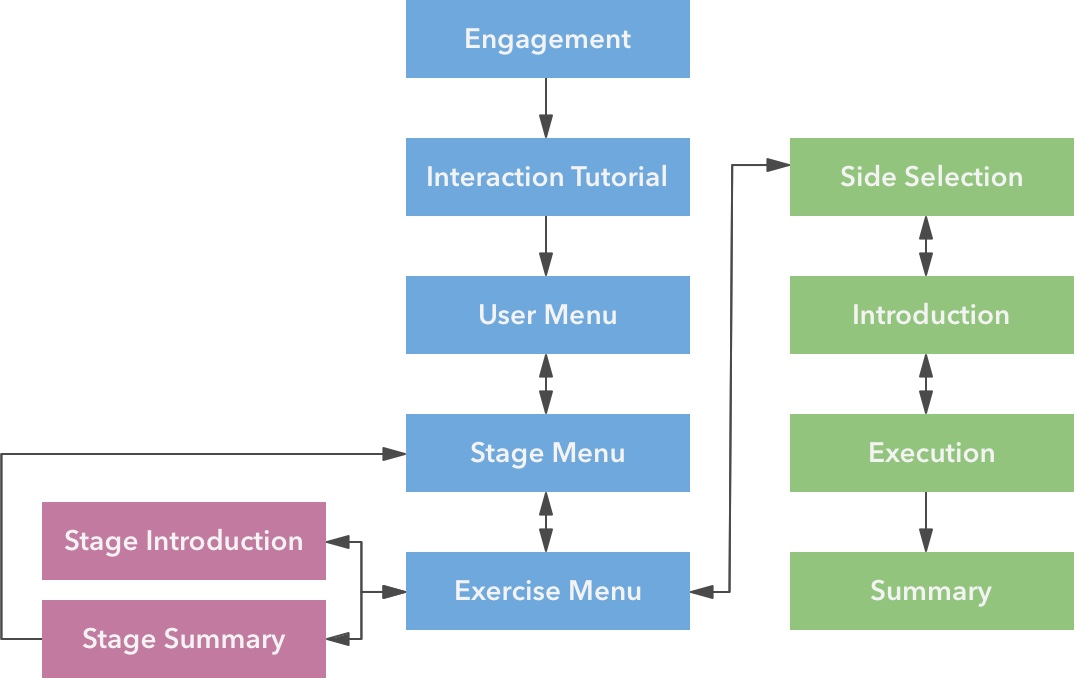
\includegraphics[width=1\linewidth]{Pictures/5_1_UIWorkflow}
		\caption{Scenario workflow}
		\label{fig:scenarioWorkflow}
	\end{minipage}
\end{figure}
